
% NOTES: Could have a section talking explicitly about the concept of the "Memory Cell"
% COuld have a section at the end that discusses choices for model parameters in a specific example
% Could have section in beginning to go over the basics of recurrent neural networks

\documentclass[journal]{IEEEtran}
\usepackage{tikz}
\usetikzlibrary{decorations.pathreplacing,angles,quotes}


% correct bad hyphenation here
\hyphenation{op-tical net-works semi-conduc-tor}

\begin{document}
%
% paper title
\title{LSTM Method Discussion Report}

% puts info about authors at bottom of first page
\author{Lawrence~Owusu,~Jordan~Sturtz,~and~Swetha~Chittam~% <-this % stops a space
  \thanks{The authors are graduate students at NCA\&T}% <-this % stops a space
}

% note the % following the last \IEEEmembership and also \thanks -
% these prevent an unwanted space from occurring between the last author name
% and the end of the author line. i.e., if you had this:
%
% \author{....lastname \thanks{...} \thanks{...} }
%                     ^------------^------------^----Do not want these spaces!

% The paper headers
% The only time the second header will appear is for the odd numbered pages
% after the title page when using the twoside option.
\markboth{CS851 - Deep Learning: Method Discussion Report}%
{Shell \MakeLowercase{\textit{et al.}}: CS851 - Deep Learning: Method Discussion Report}

% make the title area
\maketitle

% As a general rule, do not put math, special symbols or citations
% in the abstract or keywords.
% \begin{abstract}
% The abstract goes here.
% \end{abstract}

% Note that keywords are not normally used for peerreview papers.
% \begin{IEEEkeywords}
% IEEE, IEEEtran, journal, \LaTeX, paper, template.
% \end{IEEEkeywords}

% For peer review papers, you can put extra information on the cover
% page as needed:
% \ifCLASSOPTIONpeerreview
% \begin{center} \bfseries EDICS Category: 3-BBND \end{center}
% \fi

%
% For peerreview papers, this IEEEtran command inserts a page break and
% creates the second title. It will be ignored for other modes.
\IEEEpeerreviewmaketitle

\section{Summary}
%
% Here we have the typical use of a "T" for an initial drop letter
% and "HIS" in caps to complete the first word.
\IEEEPARstart{L}{ong} Short Term Memory (LSTM) is a powerful machine learning method
for learning tasks involving sequences with long-term dependencies. LSTM is a variant
of recurrent neural networks with a specialized architecture designed to solve the
vanishing gradient problem that prevents deep neural networks from learning long-term dependencies.
The original authors of LSTM, Hochreiter and Schmidhuber, designed the first variant of LSTM in 1997 that introduced
the idea of creating a unit in the neural network architecture that enforces constant error backflow [1]. To solve
the problem of conflicting weight signals, Hochreiter and Schmidhuber then added two additional features to their
model architecture: an input gate and an output gate [1]. Later, other authors would develop this architecture further
to add a "forget" gate, which is the variant of the LSTM architecture we explore in this report [2]. These gates use
a sigmoid layer together with pointwise multiplication to allow the network to filter signals.
\\

% FIXME: Not a good design pattern here to be manually entering reference numbers
% Should have an automatic method

\section{Recurrent Neural Networks}
Recurrent neural networks are neural networks that feature
feedback connections. These feedback connections typically occur when the output at time step $t$
is combined, usually concatenated, with the input for time step $t+1$ (See Fig. 1). LSTM
is a recurrent NN. Each memory block is recurrently connected to the next memory block,
which each memory block assigned to a specific timestep in the input sequence.

\begin{figure}[h]
  \centering
  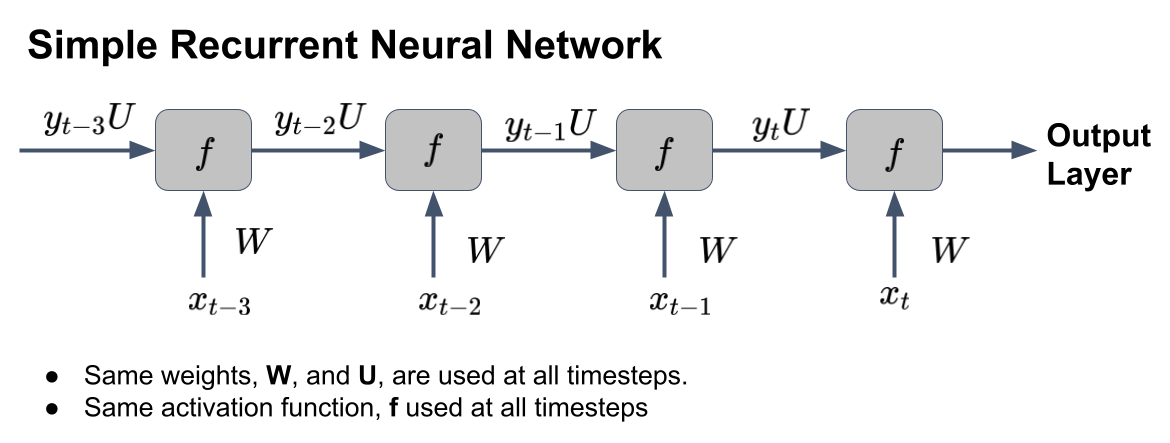
\includegraphics[width=8cm]{RNN Illustration.png}
  \caption{Typical Simple RNN Structure}
\end{figure}

\section{The LSTM Architecture}
Characteristic of the LSTM architecture is a set of chained together cells called "memory blocks". The number
of memory blocks in the chain equals the length of the timesteps in our target dataset (Fig 2).
Each memory cell has three gating units (forget, input and output gates) which
conditionally regulate how information flows into and out of the memory block (Fig 3). Intuitively,
the "forget" gate can be viewed as a step where irrelevant information from the hidden state
is first "forgotten" before being passed to the input gate, which constructs the new cell state.
Before that cell state can output its value to the next memory cell, it is filtered again through
an output gate that decides what values to keep internal to the memory cell (i.e. the hidden state)
and what to output to the next memory cell or final output layer.

\begin{figure}[h]
\centering
\tikzstyle{place}=[rectangle,draw, thick, minimum width=30, minimum height=10]
\begin{tikzpicture}
    \node at (0,0) [place] (first) {Memory Cell};
    \node at (3,0) [place] (second) {Memory Cell};
    \node at (6,0) [place] (third) {Memory Cell};
    % \draw [->] (0,0) -- (first.west);
    \draw [->] (first.east) -- (second.west);
    \draw [->] (second.east) -- (third.west);
    % \draw [->] (third.east) -- (10,0);
    \draw[decoration={brace,mirror,raise=10pt},decorate](first.south west) -- node[below=16pt] {Number of cells = number of time steps} (third.south east);
\end{tikzpicture}
\caption{Illustration of recurrently chained memory cells}
\end{figure}

% \begin{figure}[h]
%   \centering
%   \includegraphics[width=8cm]{lstm_architecture.jpeg}
%   \caption{
%   The black dots indicate a sigmoidal activation function plus pointwise multiplication to produce a "gate" that
%   filters a signal by multiplying a value between 0 and 1 to decide the strength of a signal. The center of the
%   illustration shows a linear activation function which represents the "Constant Error Carosel" of the LSTM.
%   The feedback connection has a fixed weight of 1.0 on the previous timestep, with a linear activation function of
%   $f_{j}(x) = x, \forall x$, which Hochreiter and Schmidhuber refer to as the "Constant Error Carosel".
%   Sourced from Hochreiter and Schmidhuber, p. 1744}
% \end{figure}

\begin{figure}[h]
  \centering
  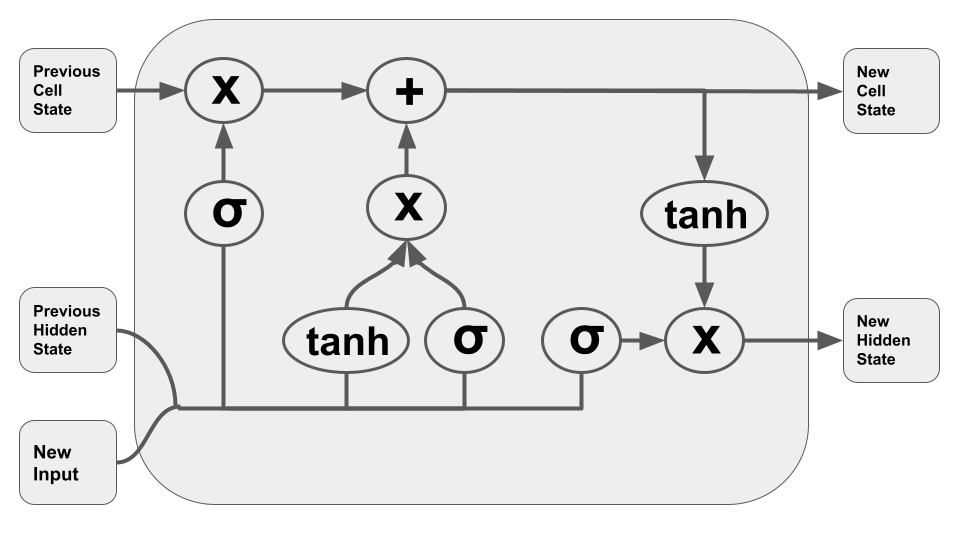
\includegraphics[width=8cm]{jordan_lstm_architecture.png}
  \caption{LSTM architecture inside a memory cell}
\end{figure}

\subsection{The Forget Gate}
The forget gate decides what information to discard from the previous hidden state given
the new input data and previous hidden state. What inputs to ignore is learned in a sigmoid-activated
neural network that is then point multipled by the previous cell state, which effectively produces a "gate" that
filters the previous cell state. The results are then passed on to the next step. The output of the forget gate
can be expressed as $f_{t} = \sigma(W_{f}h_{t-1} + U_{f}X_{t} + b_{f})$,
where $W_{f}$, $U_{f}$ are weight matrices and $b_{f}$ is a bias vector [3, p. 555].

\subsection{The Input Gate}
The input gate in the LSTM is responsible for deciding which new
information to update the cell state given the new input data and the previous hidden state.
The new cell state update can be expressed with the following equations [3, p. 555]:

$\begin{array}{ll}
C_{t}   & = f_{t} \otimes C_{t-1} + i_{t}\bar{C} \\
i_{t}   & = \sigma(W_{t}h_{t-1} + U_{i}X_{t} + b_{i}) \\
\bar{C} & = tanh(W_{c}h_{t-1} + U_{c}X_{t} + b_{c})
\end{array}$

$W_{i}$, $U_{i}$ are weight matrices and $b_{i}$ is a bias vector. $C_{t}$ is the new cell state, and the above equation
represents this new state as a pointwise addition of the previous cell state after
running through the forget gate, $f_{t}C_{t-1}$, and the result of the current input gate, $i_{t}\bar{C}$.
The equation for $i_{t}$ is the scale factor applied to the candidate that could be added to the
internal state, represented by $\bar{C}$.

\subsection{The Output Gate}
Once the cell state has been updated, the output gate decides which components of the
cell state to keep "internal" to the memory cell.
The output gate step can be expressed by the following equations [3, p. 555]:

$\begin{array}{ll}
h_{t} & = o_{t}\otimes tanh(C_{t}) \\
o_{t} & = \sigma(W_{o}h_{t-1})
\end{array}$

The current cell state, $C_{t}$ is passed to a hyperbolic tangent function, which is then pointwise multiplied
by the output gate, $o_{t}$. The output function is again another sigmoid squashing function that
acts as a filter for the output to output the new hidden state.

\ifCLASSOPTIONcaptionsoff
  \newpage
\fi

\begin{thebibliography}{1}

\bibitem{IEEEhowto:kopka}
S.~Hochreiter and J.~Schmidhuber, "Long Short-Term Memory", \emph{Neural Computation}, vol. 9, no. 8, pp. 1735-1780, 1997.
\bibitem{IEEEhowto:kopka}
F.~Gers, J.~Schmidhuber, and F.~Cummins. "Learning to forget: Continual prediction with LSTM." \emph{Neural computation}, vol. 12, no. 10, 2451-2471, 2000.
\bibitem{IEEEhowto:kopka}
O~Calin. \emph{Deep learning architectures: A mathematical approach}. Switzerland: Springer, 2020. pp. 553-547.
% \bibitem{IEEEhowto:kopka}
% R.~Williams and D.~Zipser, "Gradient-based learning algorithms for recurrent networks and their computational complexity." in \emph{Backpropagation: Theory, architectures, and applications}, pp. 433-486.
% \bibitem{IEEEhowto:kopka}
% D.~Rumelhart, G.~Hinton, and R.~Williams, "Learning representations by back-propagating errors.", \emph{Nature}, vol. 323, no. 6088, 1735-1780, 1986

\end{thebibliography}

\end{document}